\section{Gravity}
\begin{tabular*}{1.0\linewidth}{l|l}
  $M, m$ & masses of two bodies \\
  $r$    & distance between bodies
\end{tabular*}

Newton's law of gravity: the force between two bodies is $F = G\frac{Mm}{r^2}$, where $G$ is the
gravitational constant.

Units: since $[F] = \frac{LM}{T^2}$, we have $[G] = \frac{LM}{T^2}\frac{L^2}{M^2} = \frac{L^3}{MT^2}$.

\begin{tabular*}{1.0\linewidth}{l|l}
  $M_E = 5.972 \times 10^{24} kg$ & mass of the Earth \\
  $R =  6.371 \times 10^6 m$     & radius of the Earth \\
  $G = 6.67408 \times 10^{-11} m^3 kg^{-1} s^{-2}$        & gravitational constant\\
  $m$ & mass of an object
\end{tabular*}

The acceleration of the object due to gravity at the Earth's surface is
\begin{align*}
  g
  = \frac{F}{m}
  = G\frac{M_E}{R^2}
  = \frac{6.67408 \times 10^{-11} \times 5.972 \times 10^{24}}{(6.371 \times 10^6)^2}
  = 9.82 ms^{-2}.
\end{align*}


\section{Strategies for solving problems}
\subsection*{Units \& dimensional analysis}
\subsubsection*{}
\begin{mdframed}
  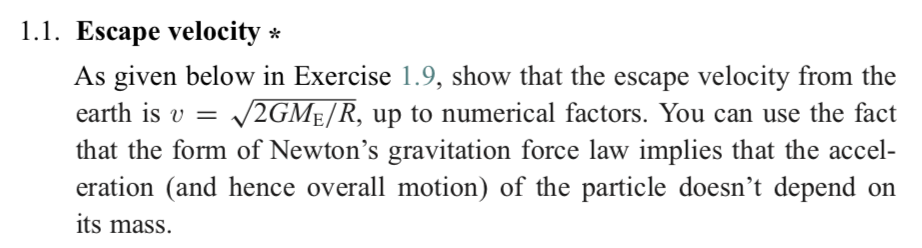
\includegraphics[width=400pt]{img/physics--classical-mechanics--morin--1-1.png}
\end{mdframed}

A projectile of mass $m$ is fired vertically upwards with velocity $v$ (no air-resistance).

When the projectile is at height $h$, the acceleration due to gravity is
$\frac{F}{m} = GM_E/(R + h)^2$, which does not depend on $m$.

We want units of $LT^{-1}$. We have

\begin{tabular*}{1.0\linewidth}{l|l}
  $[G]$        & $L^3M^{-1}T^{-2}$ \\
  $[M_E]$      & $M$ \\
  $[R]$        & $L$ \\
  $[GM_E / R]$ & $L^2T^{-2}$
\end{tabular*}

A quantity with the desired units is $\sqrt{GM_E/R}$.

More formally, suppose $v \propto G^iM_E^jR^k$.

Let  ${G, M_E, R}$ be a basis for a vector space.

Then the problem corresponds to the linear system
\begin{align*}
  \matMMMxNNN
  {3}{0}{1}
  {-1}{1}{0}
  {-2}{0}{0} \vecMMM{i}{j}{k} = \vecMMM{1}{0}{-1}.
\end{align*}
$i$ must be $1/2$, which implies $j = 1/2, k = -1/2$, i.e. $\sqrt{GM_E/R}$. \checkmark

\subsubsection*{}
\begin{mdframed}
  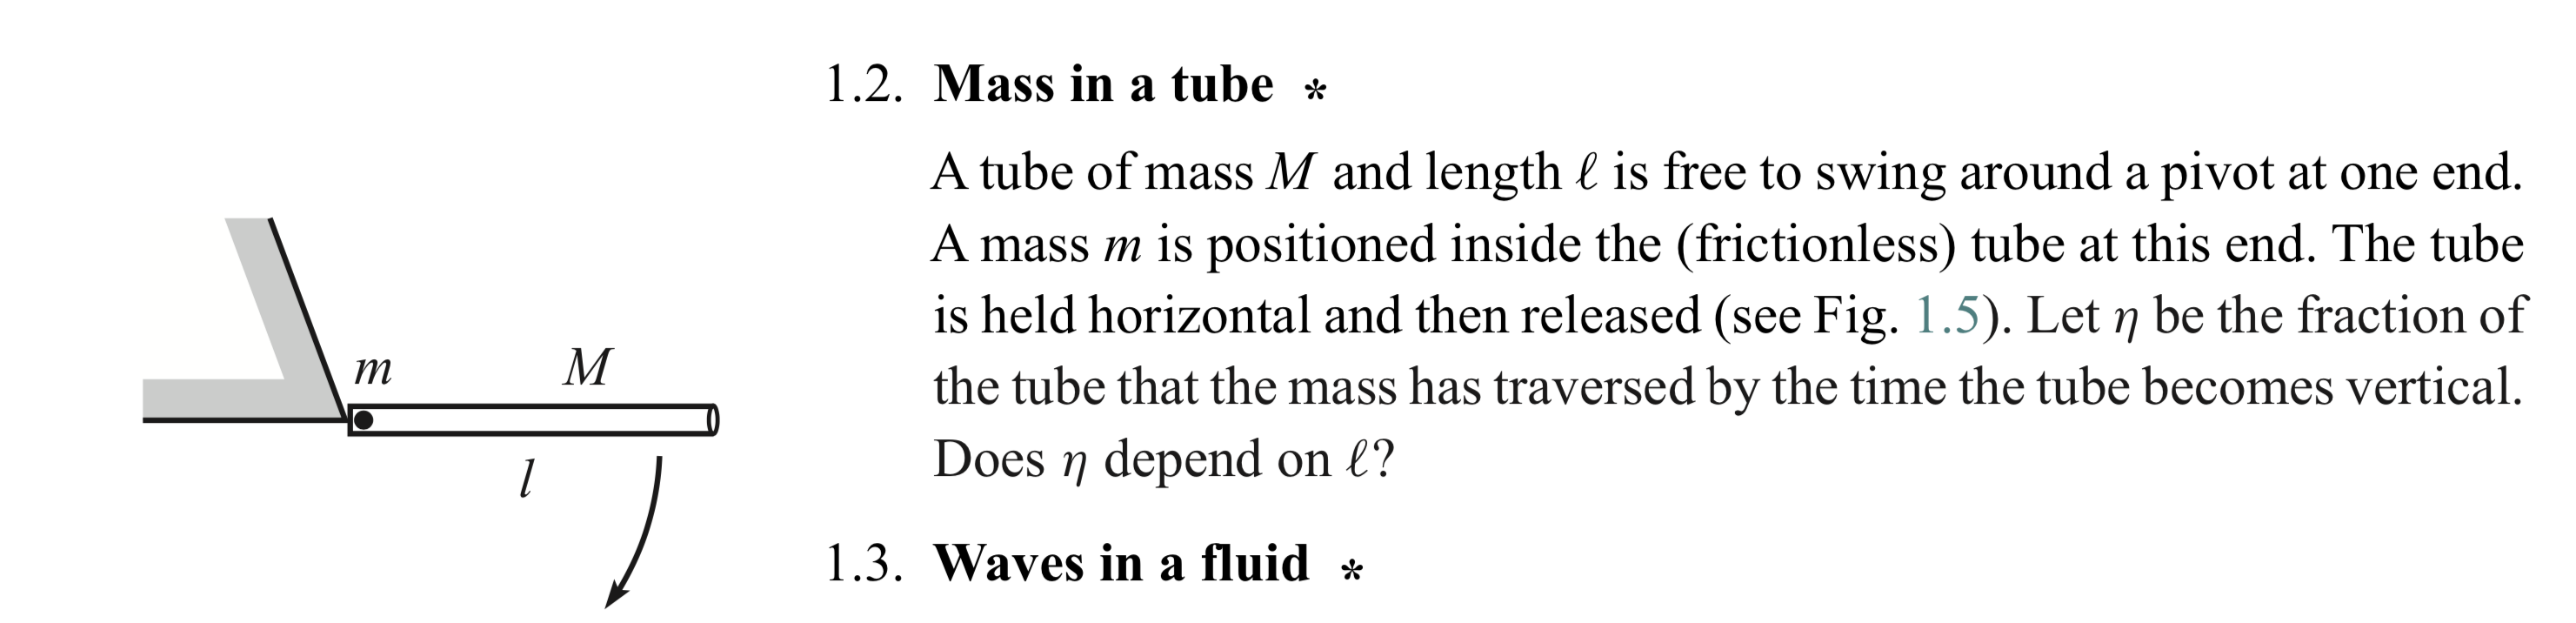
\includegraphics[width=400pt]{img/physics--classical-mechanics--morin--1-2.png}
\end{mdframed}

\begin{enumerate}
\item
  \begin{tabular}{l|l}
    $[l]$       & $L$ \\
    $[m], [M]$  & $M$ \\
    $[g]$       & $LT^{-2}$
  \end{tabular}\\
  As a fraction, $\eta$ is dimensionless. It cannot depend on $g$ since there is no other
  quantity to cancel out the time units. Suppose $\eta$ depends on some power of $l$. Then it must
  also depend on some other quantity involving distance. But there is no other
  such quantity. Therefore $\eta$ does not depend on $l$.  \checkmark

\item \todo{Why is this wrong?} We can choose an $l$ for which $\eta > 0$. Let $\eta^* > 0$ be such
  an $\eta$.

  However, as $l \to \infty$, we have $\eta \to 0$ since the distance traversed by the mass is bounded
  above by the distance the mass would drop under gravity with no opposing normal force from the tube;
  since $m$ is finite, this bound is finite.

  Therefore for all $\eta^* > 0$, we can choose an $l$ such that $\eta < \eta^*$. Therefore $\eta$
  does depend on $l$.
\end{enumerate}

\subsubsection*{}
\begin{mdframed}
  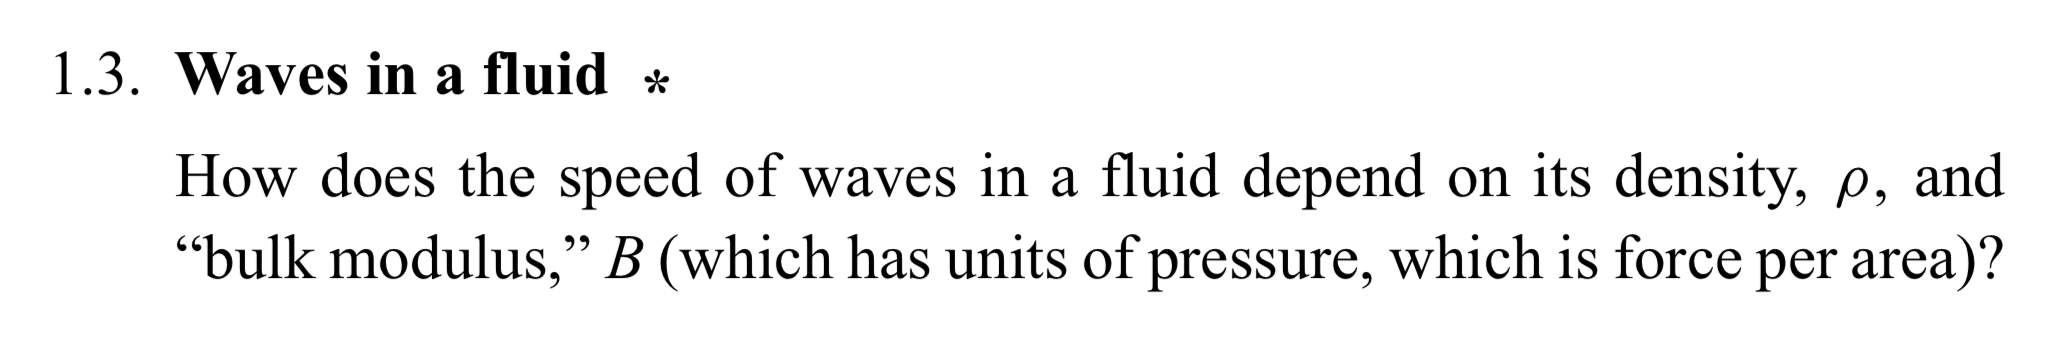
\includegraphics[width=400pt]{img/physics--classical-mechanics--morin--1-3.png}
\end{mdframed}

\begin{tabular}{l|l}
  speed   & $LT^{-1}$ \\
  density & $ML^{-3}$ \\
  bulk modulus & $MLT^{-2}L^{-2} = ML^{-1}T^{-2}$
\end{tabular}

\begin{align*}
  \matMMMxNN
  {-3}{-1}
  {1}{1}
  {0}{-2} \vecMM{i}{j} = \vecMMM{1}{0}{-1}.
\end{align*}
$\implies j = 1/2, i = -1/2$\\
So speed is proportional to $\sqrt{B/\rho}$. \checkmark

\subsubsection*{}
\begin{mdframed}
  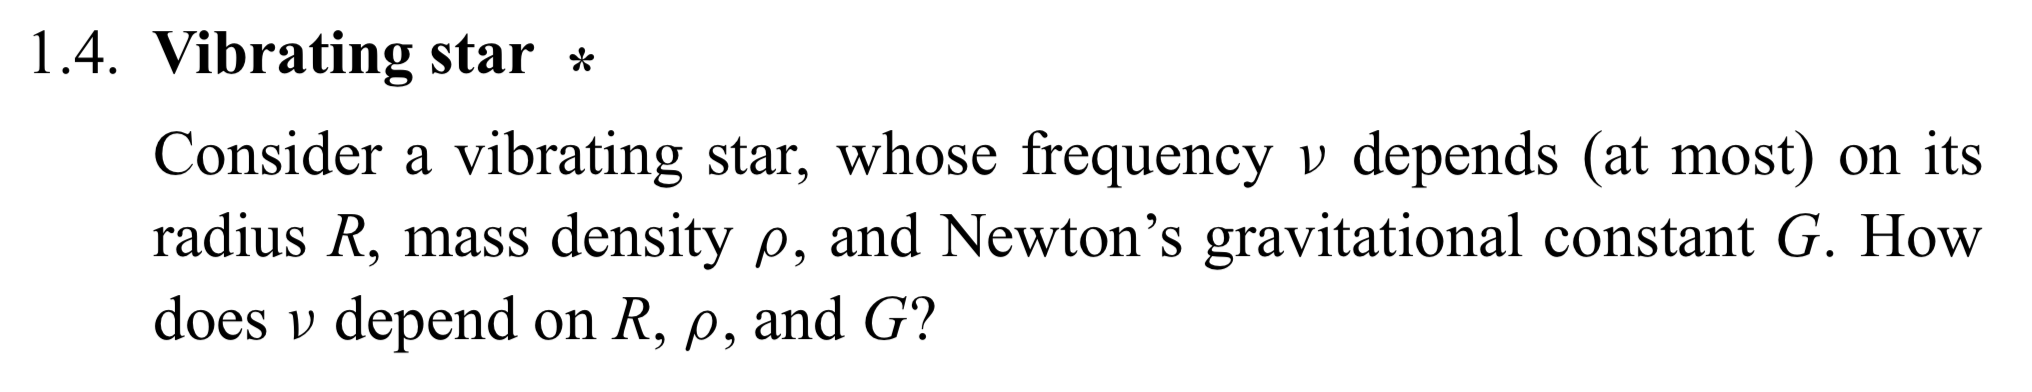
\includegraphics[width=400pt]{img/physics--classical-mechanics--morin--1-4.png}
\end{mdframed}
\begin{tabular}{l|l}
  Frequency $\nu$            & $T^{-1}$ \\
  Radius $R$                 & $L$ \\
  Mass density $\rho$        & $ML^{-3}$ \\
  Gravitational constant $G$ & $L^3M^{-1}T^{-2}$
\end{tabular}

Suppose $\nu \propto R^i\rho^jG^k$. Then $(i, j, k)^T$ would be a solution to
\begin{align*}
  \matMMMxNNN
  {1}{-3}{3}
  {0}{1}{-1}
  {0}{0}{-2} \vecMMM{i}{j}{k} = \vecMMM{0}{0}{-1}.
\end{align*}

$(0, 1/2, 1/2)$ is a solution, so frequency must be proportional to $\sqrt{G\rho}$. \checkmark

\subsubsection*{}
\begin{mdframed}
  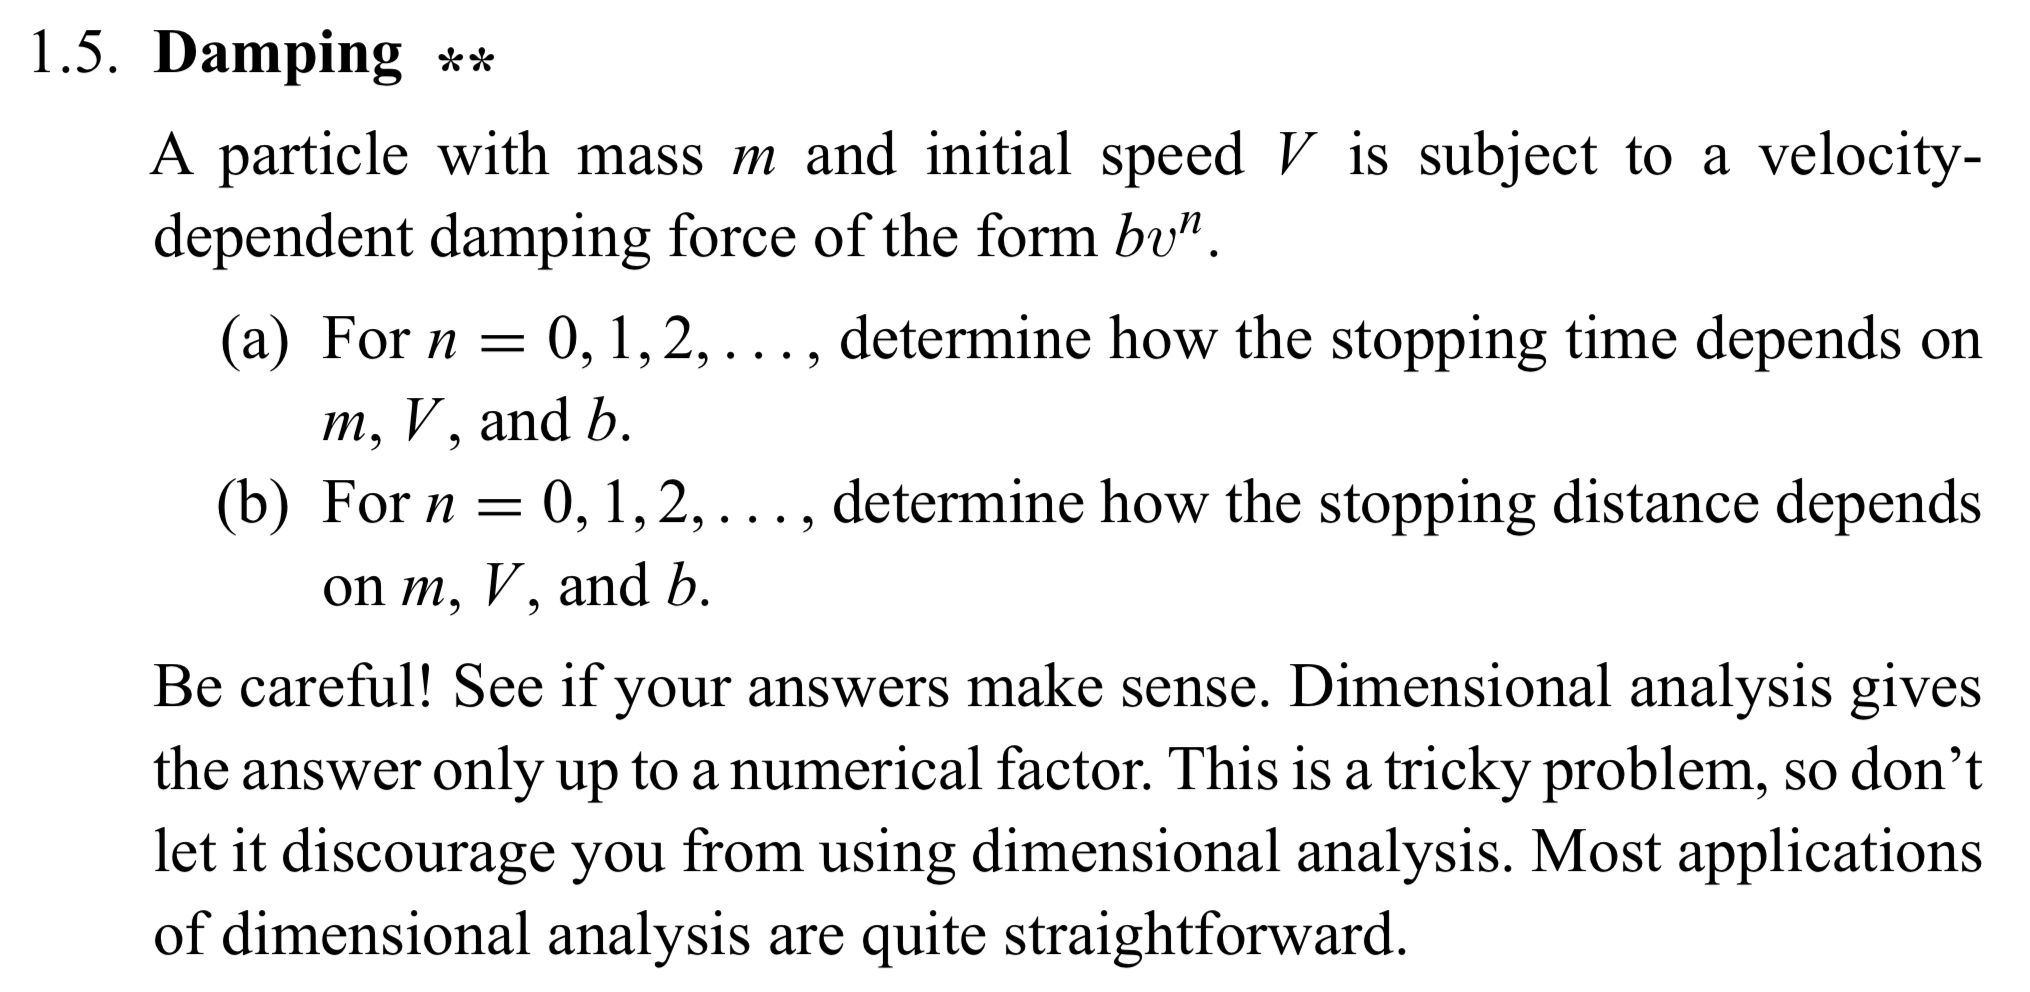
\includegraphics[width=400pt]{img/physics--classical-mechanics--morin--1-5.png}
\end{mdframed}

\begin{tabular}{l|l}
  Stopping time     & $T$ \\
  Stopping distance & $L$ \\
  \hline
  mass $m$          & $M$ \\
  Initial speed $V$ & $LT^{-1}$ \\
  Constant $b$      & $ML^{1-n}T^{n-2}$ \\
  \hline
  $v^n$             & $L^nT^{-n}$ \\
  Force $F = bv^n$  & $MLT^{-2}$
\end{tabular}

\begin{enumerate}[label=(\alph*)]
\item Stopping time\\
  Suppose $T \propto m^iV^jb^k$. Then
  \begin{align*}
    \matMMMxNNN
    {0}{1}{1-n}
    {1}{0}{1}
    {0}{-1}{n-2} \vecMMM{i}{j}{k} &= \vecMMM{0}{0}{1},
  \end{align*}
  so that
  \begin{align*}
    i + k &= 0 \\
    j + k(1 - n) &= 0 \\
    -j + k(n - 2) &= 1 \\
    k &= -1 \\
    i &= 1 \\
    j &= 1 - n.
  \end{align*}

\begin{verbatim}
#+begin_src mathematica :results pp
LinearSolve[{{0, 1, 1-n}, {1, 0, 1}, {0, -1, n-2}}, {0, 0, 1}]
#+end_src

#+RESULTS:
: {1, 1 - n, -1}
\end{verbatim}

  So we have
  \begin{align*}
    T \propto mV^{1 - n}/b.
  \end{align*}

  \begin{enumerate}
  \item $n = 0$\\
    $T \propto mV/b$. Makes sense.
  \item $n = 1$\\
    $T \propto m/b$. Why not dependent on $V$? Failure of dimensional analysis; dimensionless
    proportionality constant $f(n) = f(1) = \infty$.
  \item $n = 2$\\
    $T \propto m/(bV)$. Why decreasing with $V$? Again, $f(2) = \infty$.
  \end{enumerate}

\item Stopping distance\\
  Suppose $D \propto m^iV^jb^k$. Then
  \begin{align*}
    \matMMMxNNN
    {0}{1}{1-n}
    {1}{0}{1}
    {0}{-1}{n-2} \vecMMM{i}{j}{k} &= \vecMMM{1}{0}{0},
  \end{align*}
  so that
  \begin{align*}
    i + k &= 0 \\
    j + k(1 - n) &= 1 \\
    -j + k(n - 2) &= 0 \\
    k &= -1 \\
    i &= 1 \\
    j &= 2 - n.
  \end{align*}

\begin{verbatim}
#+begin_src mathematica :results pp
LinearSolve[{{0, 1, 1-n}, {1, 0, 1}, {0, -1, n-2}}, {1, 0, 0}]
#+end_src

#+RESULTS:
: {1, 2 - n, -1}
\end{verbatim}

  So we have
  \begin{align*}
    T \propto mV^{2 - n}/b.
  \end{align*}

  \begin{enumerate}
  \item $n = 0$\\
    $T \propto mV^2/b$. Makes sense.
  \item $n = 1$\\
    $T \propto mV/b$. Makes sense.
  \item $n = 2$\\
    $T \propto m/b$. Why not dependent on $V$?
  \end{enumerate}
\end{enumerate}

\subsection*{Approximations, limiting cases}
